\section{\emph{Docker} Infrastruktur}
Dieser Abschnitt behandelt die \emph{Docker} Infrastruktur, welche die Service und deren Abhängigkeiten \emph{hosted}. Da der Umgang mit Docker und einer umfangreicheren Infrastruktur mit viel Shell-Skripten verbunden ist, wird das Python basierte Tool \emph{Docker-Compose} verwendet, das es erlaubt eine Infrastruktur, die aus einer Menge von untereinander abhängigen Services besteht, deklarativ über eine \emph{YAML}-Konfigurationsdatei zu konfigurieren. 
\newline
\newline
Die Definition der \emph{Images} sowie der Aufbau der \emph{Docker} Infrastruktur sind im Verzeichnis \emph{$/host/docker/$} enthalten, wobei die einzelnen \emph{Dockerfiles} der Services in Unterverzeichnissen organisiert, die alle Abhängigkeiten, welche in die Images mitaufgenommen werden, enthalten. Die \emph{PostgreSQL} Images stehen am \emph{Docker Hub}\footnote{https://hub.docker.com/r/tobi312/rpi-postgresql/} zur Verfügung.   
\begin{center}
	\begin{figure}[h]
		\centering
		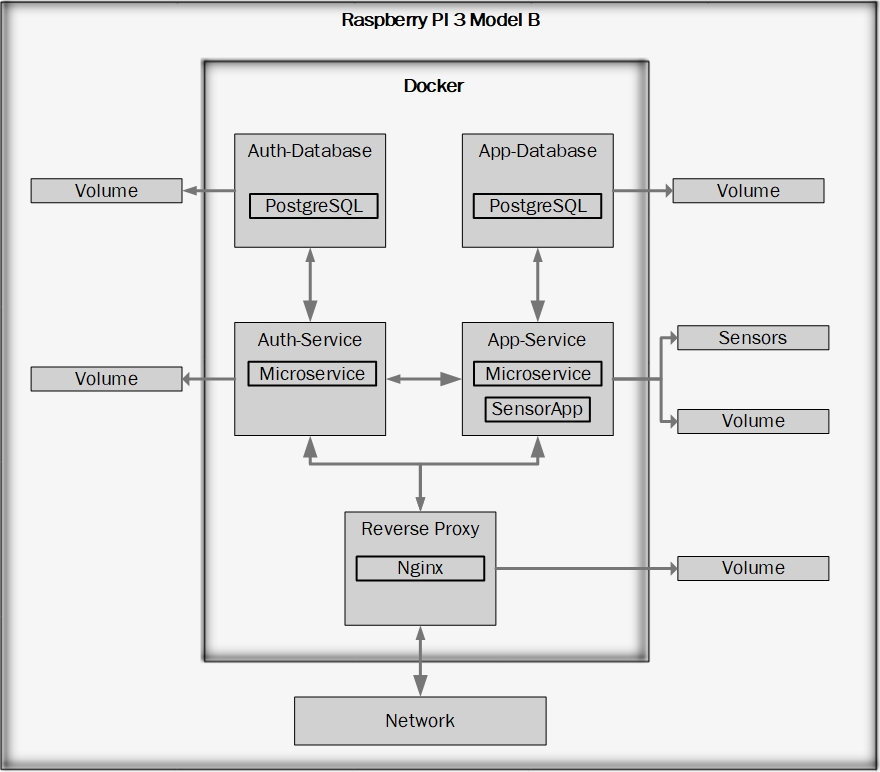
\includegraphics[scale=0.7]{\imageDir/pi-docker-infrastructure.jpg}
		\caption{\emph{Raspberry PI Docker} Infrastruktur}
		\label{fig:rapsi-docker-infrastructure}
	\end{figure}
\end{center}
Die Abbildung \ref{fig:rapsi-docker-infrastructure} zeigt die \emph{Docker} Infrastruktur, wie sie am \emph{Raspberry PI} angewendet wird. Da die Daten persistent gehalten werden müssen, werden die Daten in den \emph{Containern} in Verzeichnissen gehalten, die auf den \emph{Host} über ein \emph{Volume} gebunden sind. Der \emph{Docker Container App-Service} benötigt privilegierte Rechte damit die Sensorapplikation mit der angeschlossenen \emph{Hardware} kommunizieren kann. Die benötigten C-Bibliotheken wie \emph{WiringPI}\footnote{https://git.drogon.net/?p=wiringPi;a=summary} und die Bibliotheken für das Interagieren mit der \emph{Raspberry Pi GPU}\footnote{https://github.com/raspberrypi/userland} werden in einem Basisimage während des Bauens geladen und kompiliert. Dieses Basisimage stellt die Basis aller eigenen Images dar.
\begin{code}
	\caption{docker-compose.yml für RPISec am \emph{Raspberry PI}}
	\yamlFile{\dockerRPIDir/docker-compose.yml}
	\label{src:test-docker-compose}
\end{code}
Der Quelltext \ref{src:test-docker-compose} zeigt den Inhalt der \emph{docker-compose.yml}, welche die \emph{Docker} Infrastruktur für \emph{RPISec} am \emph{Raspberry PI} definiert. Die in der Datei vorkommenden Textfragmente im Format \emph{\$\{...\}} stellen Variablen dar, die \emph{Docker-Compose} entweder aus einer Datei mit dem Namen \emph{.env}, die auf derselben Ebene wie die \emph{docker-compose.yml} platziert werden muss, oder aus den Umgebungsvariablen des Benutzers, mit dem die Infrastruktur erstellt wird, auflöst. Sollten Variablen nicht auflösbar sein, so wird eine entsprechende Meldung auf die Konsole ausgegeben.
\newline
\newline
Das Bauen der Infrastruktur und Starten der Services dauert am \emph{Raspberry PI} relativ lange, da nur wenig Speicher zur Verfügung steht, es sich um eine ARM-Architektur handelt und das Speichermedium eine \emph{MicroSD} Karte ist. Ebenso ist die Performance der Services nicht herausragend, jedoch kann die Applikation auf dem \emph{Raspberry PI} problemlos ausgeführt werden.  